\documentclass[a4paper,14pt]{article}
\usepackage{amsmath}
\usepackage[utf8]{inputenc} % 
\usepackage{graphicx}
\graphicspath{{img/}}
\DeclareGraphicsExtensions{.png,.jpg}
\usepackage{multicol}

\usepackage[russian]{babel} % правила переноса
\usepackage[left=2cm,right=2cm,
top=2cm,bottom=2cm,bindingoffset=0cm]{geometry} % для изменения размеров полей документа
\usepackage{commath}
\usepackage{listings}
\usepackage[framed,numbered,autolinebreaks,useliterate]{mcode}

\begin{document}

%%%%%%%%%%%%%%%%%%%%%% Титульный лист %%%%%%%%%%%%%%%%%%%%%%

\begin{titlepage}
	\newpage
	
	\begin{center}
		Санкт-Петербургский государственный политехнический 
		университет Петра Великого \\
		\vspace{1cm}
		Кафедра компьютерных систем и программных технологий\\*
%		\hrulefill
	\end{center}
	
	\vspace{8em}
	
	\begin{center}
		 Отчёт по лабораторной работе №4
	\end{center}
	
	\vspace{2.5em}

	\vspace{6em}
	\flushleft{Выполнила студентка гр.33501/3: Ивашкевич О.А.}

	\flushleft{Преподаватель: Богач Н.В.}
	\vspace{\fill}
	
	\begin{center}
		Санкт-Петербург
		
		 2017
	\end{center}
	
\end{titlepage}

\tableofcontents

\newpage

\part*{Лабораторная работа №4. Аналоговая модуляция}
\setcounter {section}{0}
\setcounter {equation}{0}
\setcounter {figure}{0}
\section{Цель работы}
\hspace{0,5cm}  Изучение амплитудной модуляции/демодуляции сигнала.
\section{Постановка задачи}
\begin{enumerate}
\item Сгенерировать однотональный сигнал низкой частоты.
\item Выполнить амплитудную модуляцию (АМ) сигнала для различных значений глубины модуляции M.
\item Получить спектр модулированного сигнала.
\item Выполнить модуляцию с подавлением несущей. Получить спектр.
\item Выполнить однополосную модуляцию
\item Выполнить синхронное детектирование и получить исходный однополосный сигнал.
\item Рассчитать КПД модуляции.
\end{enumerate}

\section{Теоретическое обоснование}

\hspace{0,5cm}При создании систем передачи информации в большинстве случаев оказывается,что спектр исходного сигнала, подлежащего передаче, сосредоточен отнюдь не на тех частотах, которые эффективно пропускает имеющийся канал связи. Кроме того, очень часто необходимо в одном и том же канале связи передавать несколько сигналов одновременно. Одним из способов решения этой задачи является использование частотного разделения каналов, при котором разные сигналы занимают неперекрывающиеся полосы частот.

\hspace{0,5cm}Далее, во многих случаях требуется, чтобы передаваемый сигнал был узкополосным. Это означает, что эффективная ширина спектра намного меньше его центральной частоты:

\[\delta f << f_0.\]

\hspace{0,5cm}Перечисленные причины приводят к необходимости такой трансформации исходного сигнала, чтобы требования, предъявляемые к занимаемой сигналом полосе частот, были выполнены, а сам исходный сигнал можно было восстановить.

\hspace{0,5cm}Решение указанной проблемы достигается при использовании модуляции (modulation), сущность которой заключается в следующем. Формируется некоторое колебание, называемое несущим колебанием или просто несущей (carrier), и какой-либо из параметров этого колебания изменяется во времени пропорционально исходному сигналу. Исходный сигнал называют модулирующим (modulating signal), а результирующее колебание с изменяющимися во времени параметрами — модулированным сигналом (modulated signal).

\hspace{0,5cm} У гармонического сигнала общего вида есть три параметра: амплитуда, частота и начальная фаза. Каждый из них можно связать с модулирующим сигналом, получив таким образом три основных вида модуляции: амплитудную, частотную и фазовую. Частотная и фазовая модуляция очень тесно взаимосвязаны, так как обе влияют на оргумент функции cos. Поэтому два вида модуляции имеют общее название - угловая модуляция.

\hspace{0,5cm} В современных системах передачи цифровой информации также получила распространение квадратурная модуляция, при которой одновременно изменяются амплитуда и фаза сигнала.

\hspace{0,5cm}Обратный процесс — выделение модулирующего сигнала из модулированного колебания — называется \textbf{демодуляцией} (demodulation).

\subsection{Однотональная AM}
\hspace{0,5cm}При амплитудной модуляции (AM) в соответствии с модулирующим сигналом изменяется амплитуда несущего колебания:

\[
	S_{AM}(t) = (A_0 + ks_M(t)) cos(\omega_0t+\phi_0).
\]

\hspace{0,5cm}Отношение между амплитудами модулирующего сигнала Ам и несущего колебания А0 называется коэффициентом модуляции или глубиной модуляции:

\[
	m=\frac{A_M}{A_0}.
\]
\hspace{0,5cm}Обычно коэффициент модуляции должен лежать в диапазоне 0...1. При т > 1
имеет место перемодуляция (рис.1). Амплитудная огибающая при перемодуляции искажается.
\begin{figure}[bh]
	\noindent\centering{
		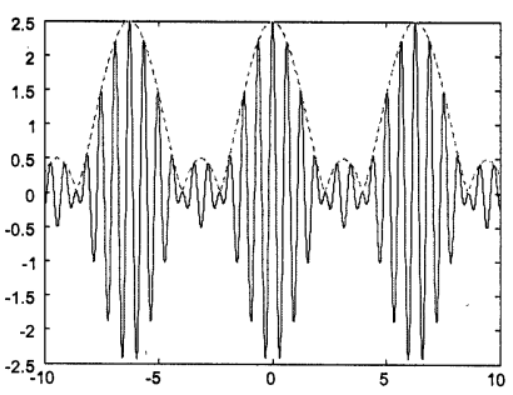
\includegraphics[width=100mm]{per}}
	\caption{Однотональный АМ-сигнал в случае перемодуляции (m=1,5)}
	\label{figCurves}
\end{figure}

\subsection{Энергетические соотношения в АМ-сигнале}

\hspace{0,5cm}Для начала определим пиковую мощность однотонального АМ-сигнала. Его максимальная амплитуда равна А0(1 + т), следовательно, пиковая мощность составляет

\[
	P_{max} = A_0^2 (1 + m)^2.
\]

\hspace{0,5cm} АМ-сигнал в общем случае не является периодическим, поэтому для расчета средней мощности необходимо применить предельный переход. Тогда средняя мощность АМ-сигнала составляет:

\[
	P_{ср} = \frac{A_0^2}{2} + \frac{A_0^2 m^2}{4}.
\]

\hspace{0,5cm}Первое слагаемое не зависит от коэффициента модуляции и представляет собой
мощность немодулированной несущей. Полезная мощность, заключенная в боковых частотах, представлена вторым слагаемым.

\hspace{0,5cm}Введем в рассмотрение коэффициент полезного действия (КПД) амплитудной модуляции, определив его как отношение мощности боковых частот к общей
средней мощности сигнала:

\[
	n_{AM} = \frac{m^2}{m^2+2} .
\]

\hspace{0,5cm}Для однополосной АМ даже при максимально допустимом значении коэффициента модуляции (m = 1) КПД составляет лишь 33 \% , то есть две трети мощности тратится на передачу бесполезной в информационном отношении несущей.

\subsection{Демодуляция AМ}

\hspace{0,5cm}Демодуляция АМ-сигнала может быть выполнена несколькими способами.
Простейший путь — имитировать работу аналогового двухполупериодного детектора. Мы вычисляем модуль входного АМ-сигнала, а затем сглаживаем получившиеся однополярные косинусоидальные импульсы, пропуская их через ФНЧ. Данный способ, очевидно, не будет работать правильно в случае перемодуляции.

\hspace{0,5cm}Следующий метод — так называемое синхронное детектирование, суть которого
состоит в умножении частоты сигнала на опорное колебание с несущей частотой:

\begin{equation}
	y(t) = \frac{1}{2} A(t) + \frac{1}{2}A(t)cos(2\omega_0t+2\phi_0).
\end{equation}

\hspace{0,5cm}Результат умножения содержит два слагаемых. Первое - это искомая
амплитудная функция, второе — АМ-сигнал с несущей частотой $2\omega_0$. Этот
высокочастотный сигнал легко удаляется путем пропускания сигнала через ФНЧ.

\hspace{0,5cm}Достоинством синхронного детектирования является то, что оно позволяет
правильно демодулировать сигнал даже в случае перемодуляции.

\subsection{AM с подавленной несущей}

\hspace{0,5cm}Для повышения КПД амплитудной модуляции можно удалить бесполезное несущее колебание, отказавшись от добавления постоянной составляющей к модулирующему сигналу. Такой способ называется AM с подавленной несущей:

\begin{equation}
	S(t) = S_M(t)*cos(\omega_0t + \phi_0).
\end{equation}

\hspace{0,5cm}Энергетический выигрыш при этом велик (КПД становится равным 100 %).

\hspace{0,5cm}Ширина спектра АМ-сигнала с подавленной несущей такая же, как в случае обычной AM (ведь подавлена средняя (несущая) частота, а боковые частоты
остались на месте).

\hspace{0,5cm}Таким образом, AM с подавленной несущей обладает определенными
преимуществами по сравнению с обычной AM. Однако этот способ модуляции не получил широкого распространения, и связано это с проблемами, возникающими при демодуляции сигнала.

\hspace{0,5cm}Демодуляция АМ с подавленной несущей может выполняться путем синхронного детектирования. При этом сохраняет силу все сказанное о необходимости точного соответствия частот и начальных фаз несущего и опорного
колебаний.

\hspace{0,5cm}Для облегчения правильного восстановления несущей иногда применяют
следующий прием. На передающей стороне несущее колебание подавляется не
полностью. Его «остаток» с небольшой амплитудой (он называется пилот-сигналом)используют для синхронизации частоты и фазы несущего колебания на
приемной стороне.

\hspace{0,5cm}Несмотря на то что визуально (на графике) однополосный сигнал сильно отличается от обычного АМ-сигнала, его демодуляция возможна тем же методом
синхронного детектирования — путем умножения на опорное колебание


\subsection{Однополосная модуляция}

\hspace{0,5cm} Диапазоны двух боковых полос АМ-сигнала являются зеркальным отражением друг друга, другими словами они несут одинаковую информацию. В следствии этого одну из боковых полос можно удалить. Получившаяся модуляция называется однополосной (британский термин — single side band, SSB).

\hspace{0,5cm}В зависимости от того, какая боковая полоса сохраняется,можно говорить об
однополосной модуляции с применением верхней или же нижней боковой полосы.

\hspace{0,5cm}Ширина спектра однополосного сигнала равна ширине спектра модулирующего сигнала. Следовательно, спектр однополосного сигнала оказывается вдвое уже, нежели при обыкновенной АМ.

\section{Ход работы}
\subsection{Однотональный сигнал низкой частоты}
Генерация гармонического сигнала и его однотональная модуляция:

\begin{lstlisting}
Fs =   2000; 
Fc = 30; 
t = 0 : 1/Fs: 2; 
A = 2;  
F = 1;
k = 1;
s = k + A * sin(2*F*pi*t); %F=1Hz
m = A/k;
n1 = m^2/(m^2+2)
x=ammod(s,Fc,Fs);
spectrum(Fs,t,x);
\end{lstlisting}

Ниже показан вид полученного модулированного сигнала во временной и частотной областях.

Для значения глубины модуляции, равной $ m = \frac{2}{2} $:

\begin{figure}[h]
\begin{multicols}{1}
\hfill
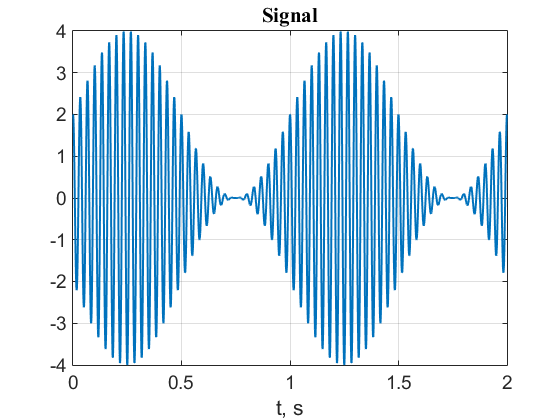
\includegraphics[width=90mm]{am1}
\hfill
\caption{Модулированный сигнал}
\label{figBottom}
\hfill
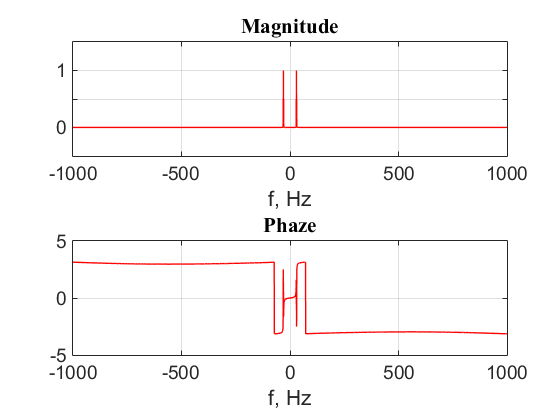
\includegraphics[width=100mm]{am1_spec}
\hfill
\caption{Спектры модулированного сигнала}
\label{figDown}
\end{multicols}
\end{figure}


Для значения глубины модуляции, равной $ m = \frac{2}{4} $:

\begin{figure}[h]
\begin{multicols}{1}
\hfill
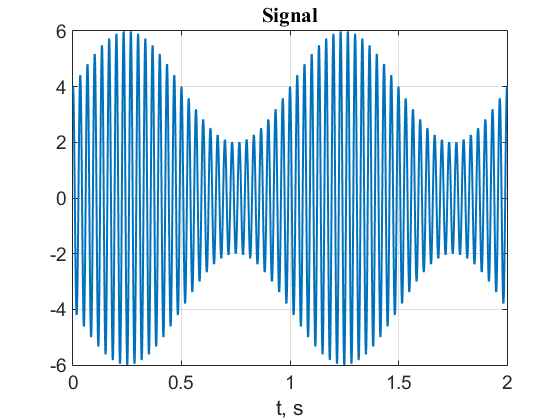
\includegraphics[width=90mm]{am1_2}
\hfill
\caption{Модулированный сигнал}
\label{figBottom}
\hfill
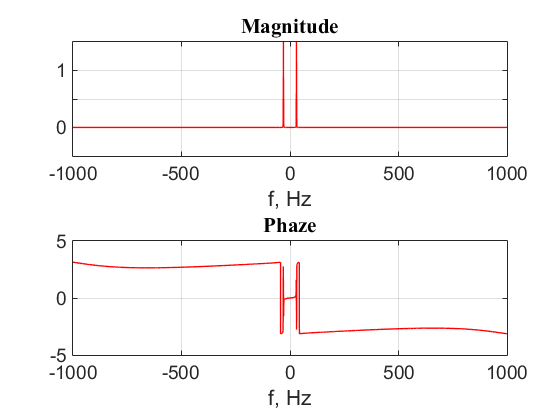
\includegraphics[width=100mm]{am1_2_spec}
\hfill
\caption{Спектры модулированного сигнала}
\label{figDown}
\end{multicols}
\end{figure}
Для значения глубины модуляции, равной $ m = \frac{1}{4} $ (недомодуляция):

\begin{figure}[h]
	\begin{multicols}{1}
		\hfill
		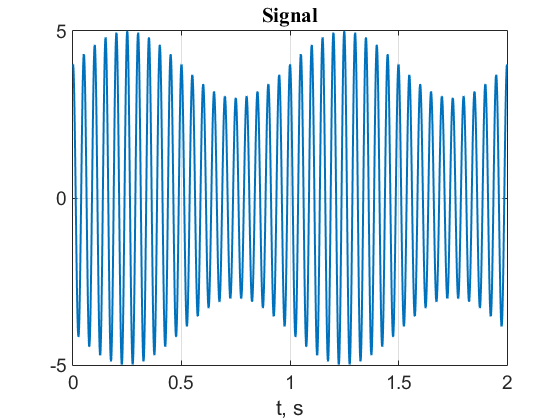
\includegraphics[width=90mm]{am1_21}
		\hfill
		\caption{Модулированный сигнал}
		\label{figBottom}
		\hfill
		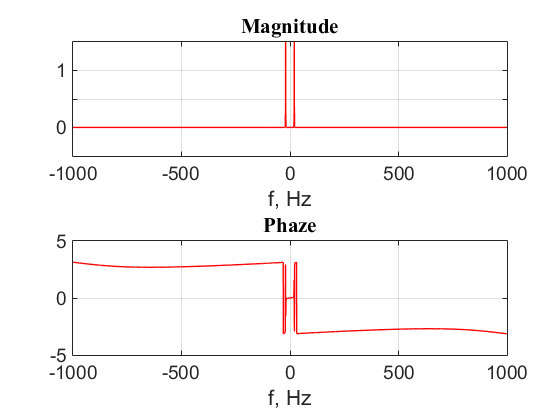
\includegraphics[width=100mm]{am1_21_spec}
		\hfill
		\caption{Спектры модулированного сигнала}
		\label{figDown}
	\end{multicols}
\end{figure}
\newpage
В связи с недомодуляцией, исходнй сигнал почти неразличим.
Для значения глубины модуляции, равной $ m = \frac{2}{1} $ (перемодуляция):

\begin{figure}[h]
\begin{multicols}{1}
\hfill
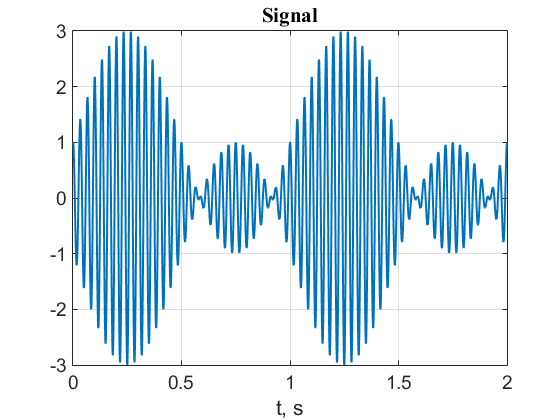
\includegraphics[width=90mm]{am1_3}
\hfill
\caption{Модулированный сигнал}
\label{figBottom}
\hfill
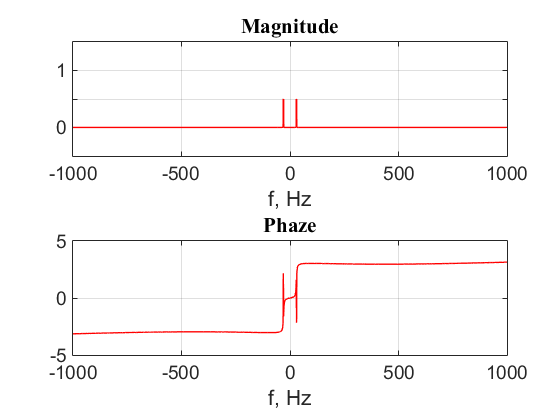
\includegraphics[width=100mm]{am1_3_spec}
\hfill
\caption{Спектры модулированного сигнала}
\label{figDown}
\end{multicols}
\end{figure}

\newpage
\subsection{Модуляция с подавлением несущей}

\begin{lstlisting}
y=ammod(s,Fc,Fs);
spectrum(Fs,t,y);
\end{lstlisting}

\begin{figure}[h]
\begin{multicols}{1}
\hfill
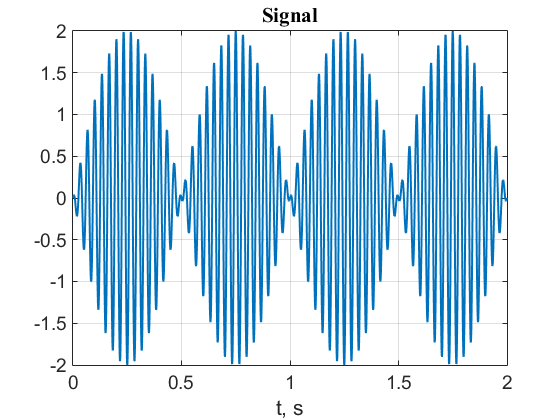
\includegraphics[width=90mm]{am2}
\hfill
\caption{Модулированный сигнал}
\label{figBottom}
\hfill
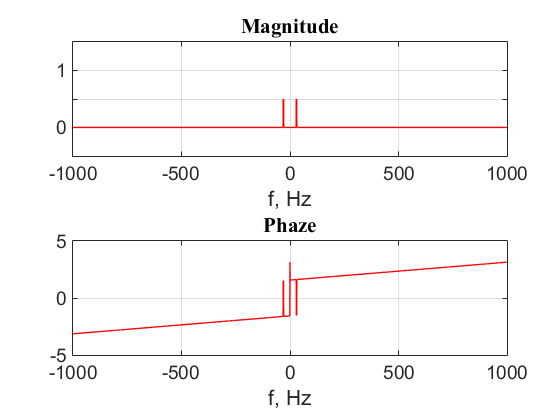
\includegraphics[width=90mm]{am2_spec}
\hfill
\caption{Спектры модулированного сигнала}
\label{figDown}
\end{multicols}
\end{figure}


\subsection{Однополосная модуляция}

Выполним однополосную модуляцию с подавлением верхней частоты:

\begin{lstlisting}
z=ssbmod(s,Fc,Fs,0,'upper');
spectrum(Fs,t,z);
\end{lstlisting}

\begin{figure}[h]
\begin{multicols}{1}
\hfill
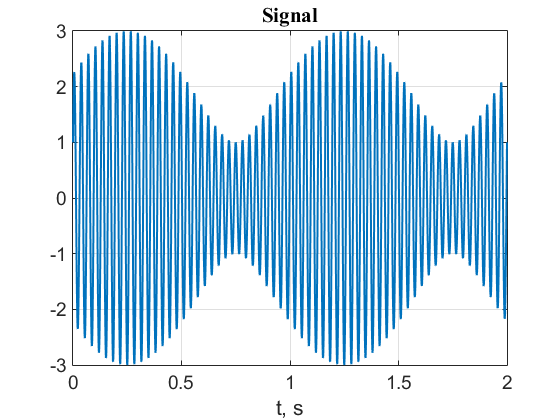
\includegraphics[width=90mm]{am4}
\hfill
\caption{Модулированный сигнал}
\label{figBottom}
\hfill
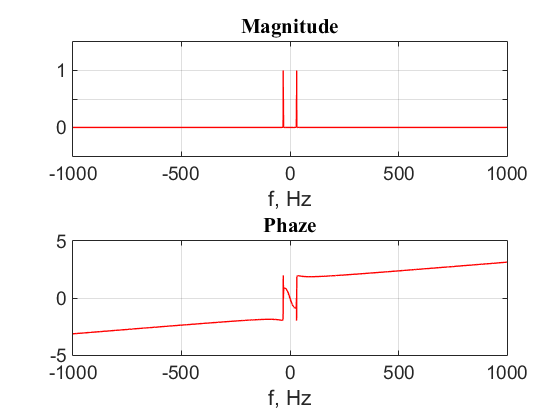
\includegraphics[width=90mm]{am4_spec}
\hfill
\caption{Спектры модулированного сигнала}
\label{figDown}
\end{multicols}
\end{figure}

\newpage
\subsection{Синхронное детектирование и получение исходного однополосного сигнала}

Выполним однополосную модуляцию с подавлением верхней частоты:

\begin{lstlisting}
z = ssbmod(s,Fc,Fs,0,'upper');
q = z.*sin(2*pi*Fc*t);
spectrum(Fs,t,q);
[b,a]=butter(5,Fc/Fs*2);
q_filt= filtfilt(b,a,q)
spectrum(Fs,t,q_filt);
\end{lstlisting}

\begin{figure}[h]
\begin{multicols}{1}
\hfill
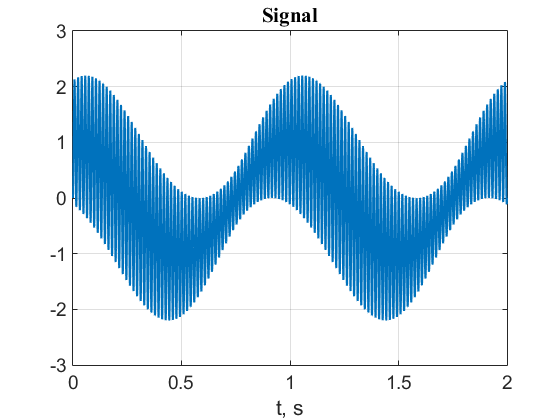
\includegraphics[width=90mm]{am5}
\hfill
\caption{Деодулированный сигнал}
\label{figBottom}
\hfill
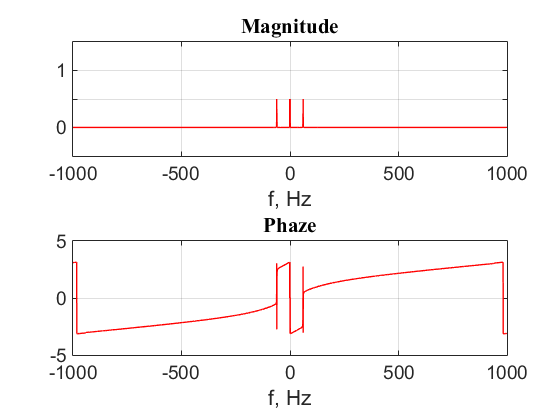
\includegraphics[width=90mm]{am5_spec}
\hfill
\caption{Спектры демодулированного сигнала}
\label{figDown}
\end{multicols}
\end{figure}


\begin{figure}[h]
\begin{multicols}{1}
\hfill
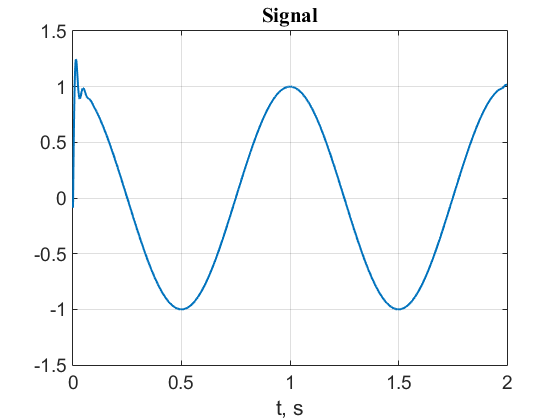
\includegraphics[width=90mm]{am6}
\hfill
\caption{Отфильтрованный сигнал}
\label{figBottom}
\hfill
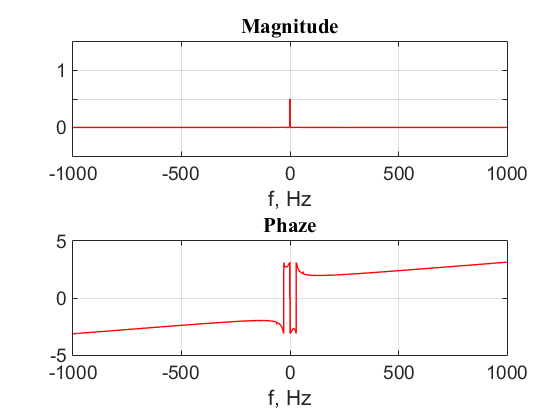
\includegraphics[width=90mm]{am6_spec}
\hfill
\caption{Спектры отфильтрованного сигнала}
\label{figDown}
\end{multicols}
\end{figure}

\newpage
\subsection{КПД модуляции}
Для каждого проделанного типа однотональной модуляции рассчитаем его КПД:
\begin{enumerate}
\item $m = 1 => n = 33\%$;
\item $m = 0.5 => n = 11\%$;
\item $m = 0.25 => n = 3\%$;
\item $m = 2 => n = 67\%$.
\end{enumerate}

\section{Выводы}
\hspace{0,5cm}
По итогам работы было получено, что КПД низкое, в следствие чего амплитудная практически не применяется. Вместо него используются частотные и фазовые модуляции, так как их КПД выше. В современном мире, амплитудная модуляция осталась лишь в радиовещании(на низких частотах) и в телевидении, для передачи изображения.
\end{document}